\documentclass[a4paper, 12pt]{article}
\usepackage[utf8]{inputenc}
\usepackage{myshortcuts}
\usepackage{a4wide}
\usepackage{csquotes}
\usepackage[british]{babel}
\usepackage[labelfont=bf]{caption}
\usepackage[style=mla,backend=biber]{biblatex}

\addbibresource{mysources.bib}

% 3011 words
\title{
\textbf{Mathematics Internal Assessment}\\
\bigskip
Is this a good title for the IA?
}
\author{Jingjie YANG}
\date{}

\begin{document}
\maketitle

\section{Introduction}\label{ch:intro}
If a large, porous stone is immersed in water for a long time, what is the probability that its centre gets wetted? In 1957, Broadbent and Hammersley \autocite*[693]{broadbent_hammersley_1957} formulated a simple stochastic model for this situation, which in two dimensions amounts to a large grid of channels. More specifically, we consider the graph $G = (V, E)$, where the set of vertices $V$ is the square lattice $\Z^2$, and all the edges that connect two neighbouring points $A$ and $B$ on the square lattice, i.e.\ $\abs{A_x - B_x} + \abs{A_y - B_y} = 1$, constitute the set of edges $E$. We then choose a certain $p \in [0, 1]$, and for each edge (alternatively called \textit{bond}) $e$ in $E$, we declare $e$ to be \textit{open} with probability $p$, and \textit{closed} otherwise with probability $1 - p$ independently of the states of other edges. This model is known as Bernoulli bond percolation.

\begin{figure}[!hb]
    \centering
    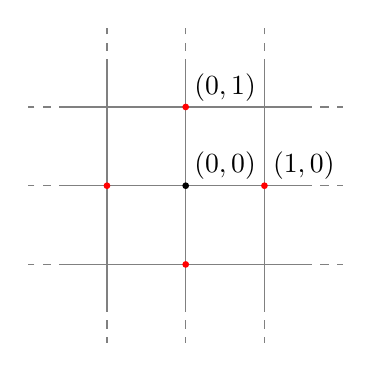
\begin{tikzpicture}
        \foreach \i in {-1, 0, 1} {
            \draw[gray] (-1.5, \i) -- (1.5, \i);
            \draw[gray] (\i, -1.5) -- (\i, 1.5);
            
            \draw[gray, dashed] (-1.5, \i) -- (-2.0, \i);
            \draw[gray, dashed] (\i, -1.5) -- (\i, -2.0);
            \draw[gray, dashed] (1.5, \i) -- (2.0, \i);
            \draw[gray, dashed] (\i, 1.5) -- (\i, 2.0);
        }
        \node at (0.5, 0.25) {$(0, 0)$};
        \node at (1.5, 0.25) {$(1, 0)$};
        \node at (0.5, 1.25) {$(0, 1)$};
        
        \filldraw (0, 0) circle (1pt);
        \filldraw[red] (0, +1) circle (1pt);
        \filldraw[red] (0, -1) circle (1pt);
        \filldraw[red] (-1, 0) circle (1pt);
        \filldraw[red] (+1, 0) circle (1pt);
    \end{tikzpicture}
    \caption{The origin (black) and its 4 neighbours (red) on the square lattice}
    \label{fig:square_lattice}
\end{figure}

The edges represent the inner passageways of the stone, where open edges let water through and closed ones block the flow; water reaches the centre of the stone if and only if the origin is in a connected component of open edges touching the boundary of the stone. In addition, it is not unreasonable to assume that the fine structure of the interior channels is on a negligible scale compared to the overall size of the stone. We are then interested in knowing whether the origin belongs to a connected component of infinitely many vertices, also called an \textit{infinite cluster}. 

Apart from $p = 0$ where the stone is entirely impermeable, and $p = 1$ where water flows surely past the origin, to have an idea of how the model behaves at other nontrivial values of $p$, we can contemplate computer simulations of a finite section of the square lattice:

\begin{figure}[!h]
    \centering
    \caption{Percolation realisations on a $16 \times 16$ section of $\Z^2$ for 3 different values of $p$}
    \label{fig:3_realisations}
    \minipage{0.32\textwidth}
    \centering
    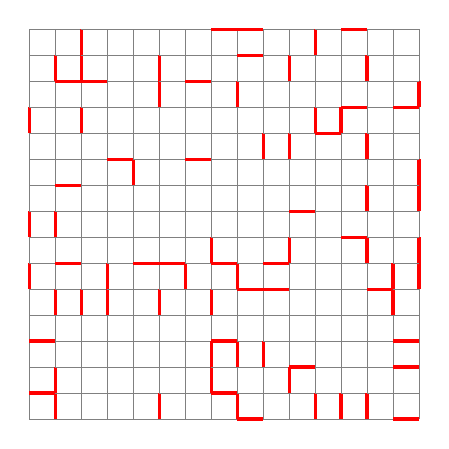
\begin{tikzpicture}
        \def\p{0.2}
        \foreach \x in {0,0.33,...,4.63} {
            \foreach \y in {0,0.33,...,4.63} {
                \pgfmathparse{rnd}
                \ifdim\pgfmathresult pt < \p pt\relax 
                    \draw[red, very thick] (\x, \y) -- (\x, \y + 0.33);
                \else
                    \draw[gray] (\x, \y) -- (\x, \y + 0.33);
                \fi 
                \pgfmathparse{rnd}
                \ifdim\pgfmathresult pt < \p pt\relax
                    \draw[red, very thick] (\x, \y) -- (\x + 0.33, \y);
                \else
                    \draw[gray] (\x, \y) -- (\x + 0.33, \y);
                \fi 
            }
            \pgfmathparse{rnd}
            \ifdim\pgfmathresult pt < \p pt\relax
                \draw[red, very thick] (\x, 4.95) -- (\x + 0.33, 4.95);
            \else
                \draw[gray] (\x, 4.95) -- (\x + 0.33, 4.95);
            \fi
            \pgfmathparse{rnd}
            \ifdim\pgfmathresult pt < \p pt\relax
                \draw[red, very thick] (4.95, \x) -- (4.95, \x + 0.33);
            \else
                \draw[gray] (4.95, \x) -- (4.95, \x + 0.33);
            \fi
        }
    \end{tikzpicture}
    \caption*{$p = 0.2$}
    \endminipage\hfill
    \minipage{0.32\textwidth}
    \centering
    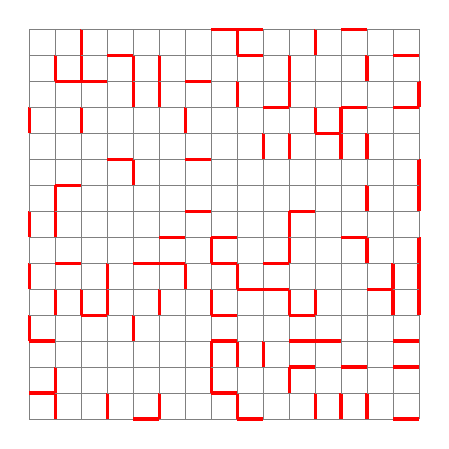
\begin{tikzpicture}
        \def\p{0.3}
        \foreach \x in {0,0.33,...,4.63} {
            \foreach \y in {0,0.33,...,4.63} {
                \pgfmathparse{rnd}
                \ifdim\pgfmathresult pt < \p pt\relax 
                    \draw[red, very thick] (\x, \y) -- (\x, \y + 0.33);
                \else
                    \draw[gray] (\x, \y) -- (\x, \y + 0.33);
                \fi 
                \pgfmathparse{rnd}
                \ifdim\pgfmathresult pt < \p pt\relax
                    \draw[red, very thick] (\x, \y) -- (\x + 0.33, \y);
                \else
                    \draw[gray] (\x, \y) -- (\x + 0.33, \y);
                \fi 
            }
            \pgfmathparse{rnd}
            \ifdim\pgfmathresult pt < \p pt\relax
                \draw[red, very thick] (\x, 4.95) -- (\x + 0.33, 4.95);
            \else
                \draw[gray] (\x, 4.95) -- (\x + 0.33, 4.95);
            \fi
            \pgfmathparse{rnd}
            \ifdim\pgfmathresult pt < \p pt\relax
                \draw[red, very thick] (4.95, \x) -- (4.95, \x + 0.33);
            \else
                \draw[gray] (4.95, \x) -- (4.95, \x + 0.33);
            \fi
        }
    \end{tikzpicture}
    \caption*{$p = 0.3$}
    \endminipage\hfill
    \minipage{0.32\textwidth}
    \centering
    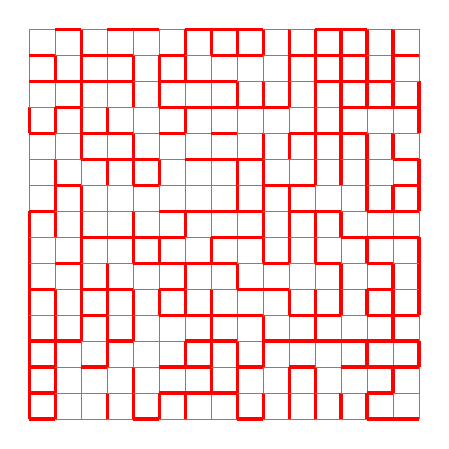
\begin{tikzpicture}
        \def\p{0.6}
        \foreach \x in {0,0.33,...,4.63} {
            \foreach \y in {0,0.33,...,4.63} {
                \pgfmathparse{rnd}
                \ifdim\pgfmathresult pt < \p pt\relax 
                    \draw[red, very thick] (\x, \y) -- (\x, \y + 0.33);
                \else
                    \draw[gray] (\x, \y) -- (\x, \y + 0.33);
                \fi 
                \pgfmathparse{rnd}
                \ifdim\pgfmathresult pt < \p pt\relax
                    \draw[red, very thick] (\x, \y) -- (\x + 0.33, \y);
                \else
                    \draw[gray] (\x, \y) -- (\x + 0.33, \y);
                \fi 
            }
            \pgfmathparse{rnd}
            \ifdim\pgfmathresult pt < \p pt\relax
                \draw[red, very thick] (\x, 4.95) -- (\x + 0.33, 4.95);
            \else
                \draw[gray] (\x, 4.95) -- (\x + 0.33, 4.95);
            \fi
            \pgfmathparse{rnd}
            \ifdim\pgfmathresult pt < \p pt\relax
                \draw[red, very thick] (4.95, \x) -- (4.95, \x + 0.33);
            \else
                \draw[gray] (4.95, \x) -- (4.95, \x + 0.33);
            \fi
        }
    \end{tikzpicture}
    \caption*{$p = 0.6$}
    \endminipage\hfill
\end{figure}
\break 

Readers with good eyesight may bother to check that for $p = 0.6$, there is a path of open edges (in red) connecting the left and right sides, whereas such is not the case for $p = 0.2$ and $p = 0.3$ where the connected components are isolated. Is there a value of the parameter $p$ at which infinite clusters emerge? Can we compute this critical value of $p$? Is the critical value different for the cubic lattice $\Z^3$?

What is described above forms the basis of percolation theory. Since its birth in 1957 due to Broandbent and Hammersley \autocite*[693]{broadbent_hammersley_1957}, the field has attracted pure mathematicians and scientists from myriad domains. Despite its simplicity, the percolation model accounts for the behaviour of many natural systems --- ranging from the flow of fluids through a disordered porous medium and conductivity of materials to the spread of forest fires and epidemics \autocite[60]{gennes_2000}. Nevertheless, the first major mathematical result was not announced until only some twenty years later: in 1980, Kesten \autocite*[41]{kesten_1980} completed Harris's \autocite*[13]{harris_lindley_1960} 1960 work to prove that the critical probability on the square lattice is equal to $\frac{1}{2}$. In the last two decades, there has been remarkable progress in our understanding of two-dimensional percolation due to Smirnov's \autocite*[239]{smirnov_2001} proof of the conformal invariance on the hexagonal lattice, for which he was awarded the Fields Medal in 2010.

To answer the questions raised above about the existence of the critical probability on the square and cubic lattices, we will firstly acquaint ourselves with a few notions in probability to allow for a rigorous discussion of the subject.

\section{Probabilistic Preliminaries}\label{ch:prelims}
We shall not get burdened with the measure-theoretic details about the probability space, but to avoid juggling with infinities in the model, some formal definitions are required.

\begin{defn}\label{defn:outcome_and_event}
We call a realisation an \textit{outcome}; e.g., the leftmost panel of \cref{fig:3_realisations} shows an outcome when $p = 0.2$. An \textit{event} is a set of zero or more outcomes, and depends on finitely many edges. We say an event \textit{occurs} if the outcome belongs to the event.
\end{defn}

\begin{ex}\label{ex:cluster_of_size_n}
Let $n$ be a nonnegative integer. Recall that a \textit{self-avoiding path} of length $n$ is a sequence of vertices $v_1, v_2, \dots, v_{n + 1}$ that are all distinct.
Let $C$ be the set of vertices that are connected to the origin $O$ via open edges (with $O \in C$). We define the event
\[
\{\abs{C} \geq n + 1\}
= \{\text{there is a self-avoiding path of open edges of length } n \text{ from } O\}
\]
where $\abs{C}$ denotes the size of the cluster $C$.
\begin{figure}[!h]
    \centering
    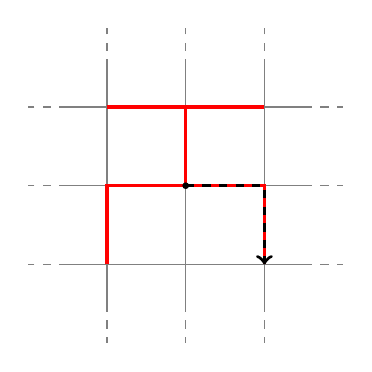
\begin{tikzpicture}
        \foreach \i in {-1, 0, 1} {
            \draw[gray] (-1.5, \i) -- (1.5, \i);
            \draw[gray] (\i, -1.5) -- (\i, 1.5);
            
            \draw[gray, dashed] (-1.5, \i) -- (-2.0, \i);
            \draw[gray, dashed] (\i, -1.5) -- (\i, -2.0);
            \draw[gray, dashed] (1.5, \i) -- (2.0, \i);
            \draw[gray, dashed] (\i, 1.5) -- (\i, 2.0);
        }
        
        \draw[red, very thick] (0, 0) -- (0, 1);
        \draw[red, very thick] (-1, 1) -- (1, 1);
        \draw[red, very thick] (-1, -1) -- (-1, 0) -- (0, 0);
        
        \draw[red, very thick] (0, 0) -- (1, 0) -- (1, -1);
        \draw[->, dashed, very thick] (0, 0) -- (1, 0) -- (1, -1);
        
        \filldraw (0, 0) circle (1pt);
        
    \end{tikzpicture}
    \caption{A self-avoiding path of length $2$ from $O$ --- the event $\abs{C} \geq 3$ occurs. }
    \label{fig:cluster_self_avoiding_path}
\end{figure}
\end{ex}

Note that we use $\P(A)$ instead of the habitual $P(A)$ to denote the probability of an event $A$ occurring, because it depends on the value of the parameter $p$. Nonetheless, the probabilities of any two events $A$ and $B$ satisfy the following as usual:
\begin{itemize}
    \item $0 \leq \P(A) \leq 1$ --- in particular, $\P(\varnothing) = 0$;
    \item $\P(A \cup B) = \P(A) + \P(B) - \P(A \cap B)$;
    \item $A$ is the \textit{complement} of $B$ if and only if $\P(A) = 1 - \P(B)$;
    \item $A$ and $B$ are \textit{independent} if and only if $\P(A \cap B) = \P(A) \P(B)$.
\end{itemize}

\begin{lem}[Monotonicity]\label{lem:event_subseteq}
If the occurrence of event $A$ implies the occurrence of event $B$, then $$\P(A) \leq \P(B).$$
\end{lem}
\begin{proof}
By \cref{defn:outcome_and_event}, we see that $A$ and $B$ are two sets of outcomes where, for all $\omega \in A$, we also have $\omega \in B$. Hence $A \subseteq B$, and 
\begin{align*}
    \P(B) 
    &= \P(A \cup (B \setminus A))\\
    &= \P(A) + \P(B \setminus A) - \P(A \cap (B \setminus A))\\
    &\geq \P(A)
\end{align*}
since $A \cap (B \setminus A) = \varnothing$ and $\P(B \setminus A) \geq 0$.
\end{proof}

\begin{cor}\label{cor:inf_cluster}
Using the definition from \cref{ex:cluster_of_size_n}, for integers $m$ and $n$, if $n > m \geq 0$, we have $\{\abs{C} \geq n\} \subseteq \{\abs{C} \geq m\}$ and hence $\P(\abs{C} \geq n) \leq \P(\abs{C} \geq m)$. We then define
\[
\P(\abs{C} = \infty) 
= \lim_{n \to \infty} \P(\text{there is a self-avoiding path of open edges of length } n \text{ from } O).
\]
\end{cor}
We also use $\theta(p)$ to refer to the probability that there is an infinite cluster at the origin as a function of $p$.

\section{Percolation on the Square Lattice}\label{sec:Z2}
\subsection{No Infinite Clusters}\label{subsec:no_inf_cluster}
To start with, we want to know for which values of $p$ (apart from $p = 0$, more specifically) there is no infinite cluster on the square lattice, i.e., $\theta(p) = 0$.

Let $n$ be a nonnegative integer, and let $\Omega_n$ be the set of all self-avoiding paths of length $n$ starting from the origin. \Cref{cor:inf_cluster} tells us that
\[\theta(p) = \lim_{n \to \infty} \P(\bigcup_{\gamma \in \Omega_n} \text{all edges of the path } \gamma \text{ are open}).\]
We can then find an upper bound on $\theta(p)$ with the help of the following lemma.

\begin{lem}[Boole's inequality]\label{lem:union_bound}
$\P(A_1 \cup A_2 \cup \cdots \cup A_n) \leq \P(A_1) + \P(A_2) + \cdots + \P(A_n)$
\end{lem}
\begin{proof}[Proof]
We proceed by induction on $n$. Let $\mathcal{P}(n): \P(\bigcup_{i = 1}^n A_i) \leq \sum_{i = 1}^n \P(A_i)$ for  $n \in \N$.
\begin{description}
\item \textit{Base case.} We have $\P(A_1) \leq \P(A_1)$, and hence $\mathcal{P}(1)$ is true.
\item \textit{Inductive step.} Assume that $\mathcal{P}(k)$ is true for a certain $k \in \N$; show that $\mathcal{P}(k + 1)$ is true.
We use the associative property of the union operation:
\begin{align*}
    \P(\bigcup_{i = 1}^{k + 1} A_i) 
    &= \P(\bigcup_{i = 1}^{k} A_i \cup A_{k + 1})\\
    &= \P(\bigcup_{i = 1}^{k} A_i) + \P(A_{k + 1}) - \P(\bigcup_{i = 1}^{k} A_i \cap A_{k + 1})\\
    &\leq \sum_{i = 1}^k \P(A_i) + \P(A_{k + 1}) - \P(\bigcup_{i = 1}^{k} A_i \cap A_{k + 1})\\
\end{align*}
Since $\P(\bigcup_{i = 1}^{k} A_i \cap A_{k + 1}) \geq 0$, we can conclude that $\P(\bigcup_{i = 1}^{k + 1} A_i) \leq \sum_{i = 1}^{k + 1} \P(A_i)$.
\end{description}
By the principle of mathematical induction, $\mathcal{P}(n)$ is true for any $n \in \N$.
\end{proof}

It follows that
\[\theta(p) \leq \lim_{n \to \infty} \sum_{\gamma \in \Omega_n} \P(\text{all edges of the path } \gamma \text{ are open}).\]

\begin{prop}\label{prop:p_path_all_open}
$\P(\text{all edges of } \gamma \text{ are open}) = p^n$ for all path $\gamma \in \Omega_n$.
\end{prop}
\begin{proof}
By the definition of the set $\Omega_n$, the self-avoiding path $\gamma$ contains $n$ distinct edges. Furthermore, each edge $e$ in $\gamma$ is defined to independently be open with probability $p$. Thus, the probability that all edges of the given path is open is $\prod_{e \in \gamma} p = p^n$.
\end{proof}

\begin{prop}\label{prop:nb_paths_len_n}
There are at most $4 \cdot 3^{n - 1}$ self-avoiding paths in $\Omega_n$.
\end{prop}
\begin{proof}
\begin{figure}[!ht]
    \centering
    \caption{Enumeration of self-avoiding paths in $\Z^2$}
    \label{fig:nb_self_avoiding_path}
    \minipage{0.5\textwidth}
    \centering
    \begin{tikzpicture}
        \foreach \i in {-1, 0, 1} {
            \draw[gray] (-1.5, \i) -- (1.5, \i);
            \draw[gray] (\i, -1.5) -- (\i, 1.5);
            \draw[gray, dashed] (-1.5, \i) -- (-2.0, \i);
            \draw[gray, dashed] (\i, -1.5) -- (\i, -2.0);
            \draw[gray, dashed] (1.5, \i) -- (2.0, \i);
            \draw[gray, dashed] (\i, 1.5) -- (\i, 2.0);
        }
        
        \filldraw (0, 0) circle (1pt);
        \draw[->, thick] (0, 0) -- (1, 0);
        \draw[->, thick] (0, 0) -- (0, 1);
        \draw[->, thick] (0, 0) -- (-1, 0);
        \draw[->, thick] (0, 0) -- (0, -1);
    \end{tikzpicture}
    \caption*{$4$ choices for the first step}
    \endminipage\hfill
    % --
    \minipage{0.5\textwidth}
    \centering
    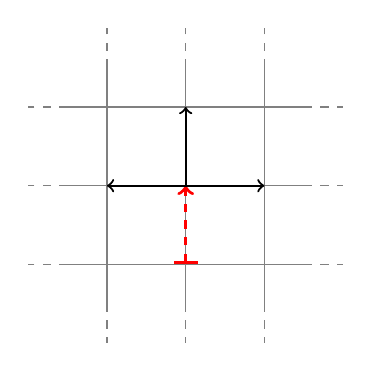
\begin{tikzpicture}
        \foreach \i in {-1, 0, 1} {
            \draw[gray] (-1.5, \i) -- (1.5, \i);
            \draw[gray] (\i, -1.5) -- (\i, 1.5);
            
            \draw[gray, dashed] (-1.5, \i) -- (-2.0, \i);
            \draw[gray, dashed] (\i, -1.5) -- (\i, -2.0);
            \draw[gray, dashed] (1.5, \i) -- (2.0, \i);
            \draw[gray, dashed] (\i, 1.5) -- (\i, 2.0);
        }
        
        \draw[|->, red, dashed, very thick] (0, -1) -- (0, 0);
        \draw[->, thick] (0, 0) -- (1, 0);
        \draw[->, thick] (0, 0) -- (0, 1);
        \draw[->, thick] (0, 0) -- (-1, 0);
    \end{tikzpicture}
    \caption*{$3$ choices for any step that follows}
    \endminipage
\end{figure}
Using the reasoning from \cref{fig:nb_self_avoiding_path} above, we can deduce that $\abs{\Omega_n} \leq 4 \times 3^{n - 1}$.
\end{proof}

\begin{thm}\label{thm:pc_lower_bound}
If $p < \dfrac{1}{3}$, then $\theta(p) = 0$.
\end{thm}
\begin{proof}
Although we have only obtained a very crude bound on the number of paths in $\Omega_n$, we can still conclude that
\begin{align*}
    \theta(p)
    &\leq \lim_{n \to \infty} \sum_{\gamma \in \Omega_n} p^n\\
    &\leq \lim_{n \to \infty} \left(4 \cdot 3^{n - 1}\right) p^n\\
    &= \dfrac{4}{3} \lim_{n \to \infty} (3p)^n
\end{align*}

The limit tends toward 0 if $\abs{3p} < 1$. Then, $p < \frac{1}{3}$ implies $\theta(p) \leq 0$. But since $\theta(p) \geq 0$ as a probability, we have $\theta(p) = 0$.
\end{proof}

As a result, there is no infinite cluster on the square lattice if $p < \frac{1}{3}$.

\subsection{Infinite Clusters}\label{subsec:inf_cluster}
Then, we are interested in knowing for which values of $p$ (other than $p = 1$) there exists an infinite cluster, i.e.\ $\theta(p) > 0$.

This time, we will be employing a more elaborated method that is often called a \textit{Peierls argument}. It is named after the British physicist who proved a phase transition --- the change of macroscopic behaviour as the parameter varies, e.g.\ the appearance of an infinite cluster --- for the Ising model, another probabilistic model in statistical physics that explains the phenomenon of ferromagnetism. The gist is that, instead of trying to directly find a lower bound on $\theta(p)$, we establish an upper bound on $1 - \theta(p)$ using a variant of the technique from the previous section. The method revolves around the \textit{dual graph} $\left(\Z^2\right)^*$, a key notion that we will introduce now.

\begin{defn}\label{defn:dual_graph}
Given a planar graph $G$, we define its \textit{dual graph} $G^*$ in such a way that:
\begin{itemize}
    \item $G^*$ has a vertex for each face delimited by edges of $G$;
    \item an edge connects two vertices of $G^*$ if the corresponding faces are separated by an edge of $G$.
\end{itemize}
\end{defn}
\begin{ex}\label{ex:dual_lattice}
Consider $\left(\Z^2\right)^*$, the dual graph of the square lattice $\Z^2$ and its edges.
\begin{figure}[h!]
    \centering
    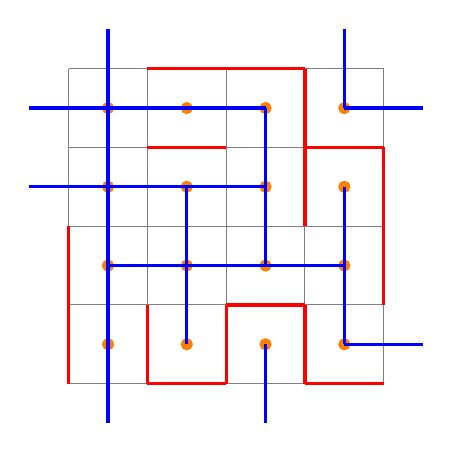
\begin{tikzpicture}
        % Grid
        \foreach \x in {0, 1, ..., 4} {
            \draw[gray] (0, \x) -- (4, \x);
            \draw[gray] (\x, 0) -- (\x, 4);
        }
        
        
        \foreach \i in {0.5, 1.5, ..., 3.5} {
            \foreach \j in {0.5, 1.5, ..., 3.5} {
                \filldraw[orange] (\i, \j) circle (2.0pt);
            }
        }
        
        % Percolation
        %% |
        \draw[red, very thick] (0, 2) -- (0, 0);
        \draw[red, very thick] (1, 1) -- (1, 0);
        \draw[red, very thick] (2, 1) -- (2, 0);
        \draw[red, very thick] (3, 4) -- (3, 2); 
        \draw[red, very thick] (3, 1) -- (3, 0);
        \draw[red, very thick] (4, 3) -- (4, 1);
        %% -
        \draw[red, very thick] (1, 4) -- (3, 4);
        \draw[red, very thick] (1, 3) -- (2, 3);
        \draw[red, very thick] (3, 3) -- (4, 3);
        \draw[red, very thick] (2, 1) -- (3, 1);
        \draw[red, very thick] (1, 0) -- (2, 0);
        \draw[red, very thick] (3, 0) -- (4, 0);
        
        % Dual percolation
        %% -
        \draw[blue, very thick] (-0.5, 3.5) -- (2.5, 3.5);
        \draw[blue, very thick] (3.5, 3.5) -- (4.5, 3.5);
        \draw[blue, very thick] (-0.5, 2.5) -- (2.5, 2.5);
        \draw[blue, very thick] (0.5, 1.5) -- (3.5, 1.5);
        \draw[blue, very thick] (3.5, 0.5) -- (4.5, 0.5);
        %% |
        \draw[blue, very thick] (0.5, 4.5) -- (0.5, -0.5);
        \draw[blue, very thick] (1.5, 2.5) -- (1.5, 0.5);
        \draw[blue, very thick] (2.5, 3.5) -- (2.5, 1.5);
        \draw[blue, very thick] (2.5, 0.5) -- (2.5, -0.5);
        \draw[blue, very thick] (3.5, 4.5) -- (3.5, 3.5);
        \draw[blue, very thick] (3.5, 2.5) -- (3.5, 0.5);
        
    \end{tikzpicture}
    \caption{A percolation realisation on a $5 \times 5$ section of the square lattice and its dual}
    \label{fig:square_lattice_dual}
\end{figure}

We observe that the graph $\Z^2$ is \textit{self-dual}: by a vector transformation of $(\frac{1}{2}, \frac{1}{2})$, each vertex (resp.\ edge) of $\Z^2$ uniquely correspond to a vertex (resp.\ edge) in $(\Z^2)^*$. Moreover, concerning percolation, we declare each edge $e^*$ of $(\Z^2)^*$ to be open (resp.\ closed) if the edge $e$ of $\Z^2$ that $e^*$ crosses is closed (resp.\ open). In other words, the event that $e^*$ is open is the complement of the event that $e$ is open. Since $e$ is open with probability $p$, the probability of $e^*$ being open is $1 - p$. As such, we consider percolation is realised in $(\Z^2)^*$ with parameter $1 - p$.

\Cref{fig:square_lattice_dual} above shows an example of how from the open edges (red) in $\Z^2$ (grey grid) we can create the dual open edges (blue) in $(\Z^2)^*$ (orange dots). Notice that, in the top-left corner, the cluster of 2 vertices in $\Z^2$ is surrounded by a cycle of open edges in $(\Z^2)^*$. We can then formulate a condition for the cluster at the origin to be finite in a similar fashion.
\end{ex}

Let $\{\abs{C} < \infty\}$ denote the event that the cluster $C$ at the origin contains finitely many vertices.

\begin{prop}\label{prop:c_finite_iff_cycle}
$\abs{C} < \infty$ if and only if there exists a cycle of open edges in $(\Z^2)^*$ surrounding $O$. Also, the cycle passes by the point $(n + \frac{1}{2}, \frac{1}{2})$ for some nonnegative $n$.
\end{prop}

This is a result from pure graph theory. We will not present the rigorous proof due to Grimett \autocite*[14--15]{grimmett_1999} here, but the reader should be able to convince him/herself that this proposition is very believable simply by drawing some pictures. Indeed, a cycle of open edges in $(\Z^2)^*$ blocks all open edges of $\Z^2$ connecting the interior and the exterior of the circuit. The cluster $C$ is then confined inside the cycle, and therefore can only contain finitely many vertices. In addition, for the cycle to surround the origin, it must intersect the line $y = \frac{1}{2}$ (which lies right above the origin) on the right, i.e., at a nonnegative $x$.

\begin{prop}\label{prop:cylce_implies_path}
Let $n$ be a nonnegative integer. If there exists a cycle in $(\Z^2)^*$ surrounding $O$ and passing by $(n + \frac{1}{2}, \frac{1}{2})$, then there exists a self-avoiding path in $(\Z^2)^*$ starting from $(n + \frac{1}{2}, \frac{1}{2})$ of length $2n + 3$.
\end{prop}
\begin{proof}
As shown in \cref{fig:shortest_cycle_dual} below, the shortest cycle passing by $(n + \frac{1}{2}, \frac{1}{2})$ that surrounds the origin has \[2\left((n + \frac{1}{2}) - (-\frac{1}{2})\right) + 2 = 2n + 4\] distinct edges.
\begin{figure}[!h]
    \centering
    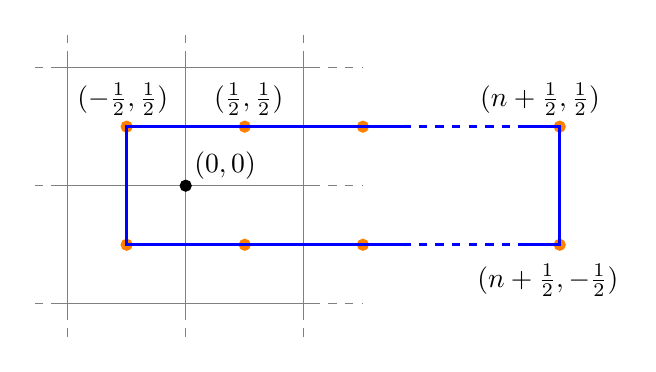
\begin{tikzpicture}
        \draw[gray] (-1.6, 1.5) -- (1.6, 1.5);
        \draw[gray] (-1.6, 0.0) -- (1.6, 0.0);
        \draw[gray] (-1.6, -1.5) -- (1.6, -1.5);
        
        \draw[gray] (-1.5, 1.6) -- (-1.5, -1.6);
        \draw[gray] (0.0, 1.6) -- (0.0, -1.6);
        \draw[gray] (1.5, 1.6) -- (1.5, -1.6);
        
        \draw[gray, dashed] (-1.5, -1.6) -- (-1.5, -2.0);
        \draw[gray, dashed] (0, -1.6) -- (0, -2.0);
        \draw[gray, dashed] (1.5, -1.6) -- (1.5, -2.0);
        
        \draw[gray, dashed] (-1.5, 1.6) -- (-1.5, 2.0);
        \draw[gray, dashed] (0, 1.6) -- (0, 2.0);
        \draw[gray, dashed] (1.5, 1.6) -- (1.5, 2.0);
        
        \draw[gray, dashed] (-1.6, 1.5) -- (-2.0, 1.5);
        \draw[gray, dashed] (-1.6, 0.0) -- (-2.0, 0.0);
        \draw[gray, dashed] (-1.6, -1.5) -- (-2.0, -1.5);
        
        \draw[gray, dashed] (1.6, 1.5) -- (2.25, 1.5);
        \draw[gray, dashed] (1.6, 0.0) -- (2.25, 0.0);
        \draw[gray, dashed] (1.6, -1.5) -- (2.25, -1.5);
        
        % Origin
        \node at (0.5, 0.25) {$(0, 0)$};
        \filldraw (0, 0) circle (2.0pt);
        
        % Dual
        \filldraw[orange] (0.75, 0.75) circle (2pt);
        \filldraw[orange] (0.75, -0.75) circle (2pt);
        \filldraw[orange] (-0.75, 0.75) circle (2pt);
        \filldraw[orange] (-0.75, -0.75) circle (2pt);
        
        \filldraw[orange] (2.25, 0.75) circle(2pt);
        \filldraw[orange] (2.25, -0.75) circle(2pt);
        
        \filldraw[orange] (4.75, 0.75) circle(2pt);
        \filldraw[orange] (4.75, -0.75) circle(2pt);
        
        \node at (0.8, 1.10) {$(\frac{1}{2}, \frac{1}{2})$};
        \node at (-0.8, 1.10) {$(-\frac{1}{2}, \frac{1}{2})$};
        \node at (4.5, 1.10) {$(n + \frac{1}{2}, \frac{1}{2})$};
        \node at (4.6, -1.20) {$(n + \frac{1}{2}, -\frac{1}{2})$};
        
        % Cycle
        \draw[blue, very thick] (4.25, -0.75) -- (4.75, -0.75) -- (4.75, 0.75) -- (4.25, 0.75);
        \draw[blue, very thick] (2.75, -0.75) -- (-0.75, -0.75) -- (-0.75, 0.75) -- (2.75, 0.75);
        \draw[blue, very thick, dashed] (2.75, -0.75) -- (4.25, -0.75);
        \draw[blue, very thick, dashed] (2.75, 0.75) -- (4.25, 0.75);
    \end{tikzpicture}
    \caption{The shortest cycle in $(\Z^2)^*$ passing by $(n + \frac{1}{2}, \frac{1}{2})$ and surrounding $O$}
    \label{fig:shortest_cycle_dual}
\end{figure}

Recall from graph theory that a cycle has no repeated edges or repeated vertices except for the starting and ending ones. By definition, a cycle without the last vertex is a self-avoiding path. Since all cycles passing by $(n + \frac{1}{2}, \frac{1}{2})$ contain at least $2n + 4$ edges, it must also contain a self-avoiding path starting from $(n + \frac{1}{2}, \frac{1}{2})$ that is of length $2n + 3$.
\end{proof}

\begin{thm}\label{thm:pc_higher_bound}
If $p > 0.762$, then $\theta(p) > 0$.
\end{thm}
\begin{proof}
We begin by finding an upper bound on the probability that $\abs{C}$ is finite.
\begin{align}
    \P(\abs{C} < \infty)
    &= \lim_{N \to \infty} \P\left(\bigcup_{n = 0}^N \exists\,\text{cycle surrounding the origin passing by } (n + \frac{1}{2}, \frac{1}{2})\right)\label{eq:union_exists_cycle}\\
    &\leq \lim_{N \to \infty} \sum_{n = 0}^N \P\left(\exists\,\text{cycle surrounding the origin passing by } (n + \frac{1}{2}, \frac{1}{2})\right)\label{eq:sum_exists_cycle}\\
    &\leq \lim_{N \to \infty} \sum_{n = 0}^N \P(\bigcup_{\gamma \in \Omega_{2n + 3}} \text{all edges of the path } \gamma \text{ are open})\label{eq:sum_union_exists_path}\\
    &\leq \lim_{N \to \infty} \sum_{n = 0}^N \sum_{\gamma \in \Omega_{2n + 3}} \P(\text{all edges of the path } \gamma \text{ are open})\label{eq:sum_sum_path_open}\\
    &\leq \lim_{N \to \infty} \sum_{n = 0}^N (4 \cdot 3^{2n + 2}) (1 - p)^{2n + 3}\label{eq:sum_path_open}
\end{align}
We start by using the equivalence between the event $\{\abs{C} < \infty\}$ and the existence of a cycle in $(\Z^2)^*$ around the origin stated in \cref{prop:c_finite_iff_cycle} to establish \cref{eq:union_exists_cycle}. Next, \cref{lem:union_bound} allows us to express the probability of a union of events as the sum of the probabilities of the events in \cref{eq:sum_exists_cycle}. Before passing to \cref{eq:sum_union_exists_path}, we need to make several observations. Firstly, we can apply \cref{lem:event_subseteq}, which allows the probability of an event to be bounded from above by the probability of another event that it implies, to find an upper bound on the probability of such cycles existing using the probability of that self-avoiding paths of a certain length exist by \cref{prop:cylce_implies_path}. In addition, the number of such paths does not depend on the starting vertex, whether it is the origin or an arbitrary $(n + \frac{1}{2}, \frac{1}{2})$; we can thus use the set $\Omega_{2n + 3}$ from \cref{subsec:no_inf_cluster}. Now, the reader should be familiar with the remaining steps, since we almost replicated them from the proof of \cref{thm:pc_lower_bound}. To derive \cref{eq:sum_sum_path_open}, we again leverage \cref{lem:union_bound} to rid of the union. Finally, in \cref{eq:sum_path_open}, we expand the sum with the upper bound on $\abs{\Omega_{2n + 3}}$ that we established in \cref{prop:nb_paths_len_n}. The only difference is that in $(\Z^2)^*$, each edge is open with probability $1 - p$ as defined in \cref{ex:dual_lattice}; we simply need to adapt \cref{prop:p_path_all_open} so that $1 - p$ is considered as the parameter instead.

We continue by considering the limit
\begin{align*}
    &\phantom{=}\lim_{N \to \infty} \sum_{n = 0}^N (4 \cdot 3^{2n + 2}) (1 - p)^{2n + 3}\\
    &= 4 \cdot 3^2 (1 - p)^3 \lim_{N \to \infty} \sum_{n = 0}^N \left(3 (1 - p)\right)^{2n}\\
    &= 36 (1 - p)^3 \lim_{N \to \infty} \sum_{n = 0}^N \left(9 (1 - p)^2\right)^n.
\end{align*}
The geometric series only converges when $\abs{9 (1 - p)^2} < 1$, i.e., when $-\frac{1}{3} < (1 - p) < \frac{1}{3}$. Since we specified that $p \in [0, 1]$, when $p > \frac{2}{3}$, the limit evaluates to
\[
    \frac{36 (1 - p)^3}{1 - 9 (1 - p)^2}.
\]

\begin{figure}[H]
    \centering
    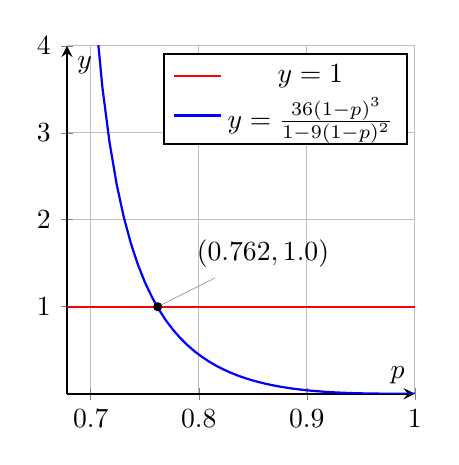
\begin{tikzpicture}
    \begin{axis}
    [xlabel={$p$}, 
     ylabel={$y$},
     axis lines=middle,
     grid,
     thick,
     domain=0.678:1,
     width=6cm,
     height=6cm,
     samples=50,
     ymin=0,
     ymax=4,
     %legend pos=outer north east
    ]
    \addplot+[no marks, red] {1};
    \addlegendentry{$y = 1$}
    \addplot+[no marks, blue] {(36 * (1-x)^3) / (1 - 9*(1-x)^2)};
    \addlegendentry{$y = \frac{36(1-p)^3}{1 - 9(1 - p)^2}$}
    \node[circle, fill=black, scale=0.35, pin=45:{$(0.762, 1.0)$}] at (axis cs:0.762, 1.0) {};
    \end{axis}
    \end{tikzpicture}
    \caption{The upper bound for $\P(\abs{C} < \infty)$}
    \label{fig:pc_upper_bound_plot}
\end{figure}

As shown in \cref{fig:pc_upper_bound_plot} above, graphically we can determine that for $p > 0.762$, \[\P(\abs{C} < \infty) \leq \frac{36(1 - p)^3}{1 - 9(1 - p)^2} < 1.\]

Note that the event $\{\abs{C} < \infty\}$ is the complement of the event $\{\abs{C} = \infty\}$, and hence
\[
    \P(\abs{C} < \infty) = 1 - \P(\abs{C} = \infty) = 1 - \theta(p).
\]

We can now conclude that
\begin{align*}
    1 - \theta(p) < 1\\
    \theta(p) > 0
\end{align*}
when $p > 0.762$.
\end{proof}

In consequence, there exists an infinite cluster on the square lattice if $p > 0.762$.

\subsection{The Critical Value}\label{subsec:pc}
Having seen how there is no infinite cluster on the square lattice when $p$ is close to $0$ and how there exists an infinite cluster when $p$ is close to $1$, via both computer simulations and mathematical proofs, it is now natural to define the critical probability $p_c$.

\begin{defn}\label{defn:pc}
The critical probability $p_c$ is a value in $[0, 1]$ such that
\[
\begin{cases}
\theta(p) = 0 &\text{if } p < p_c,\\
\theta(p) > 0 &\text{if } p > p_c.
\end{cases}
\]
\end{defn}

Moreover, in \cref{subsec:no_inf_cluster,,subsec:inf_cluster}, we have shown that $\theta(p) = 0$ if $p < \frac{1}{3}$ and $\theta(p) > 0$ if $p > 0.762$. It follows that $\frac{1}{3} \leq p_c \leq 0.762$. 

Clearly, the value of $p_c$ is not trivial --- our efforts were not in vain. That said, we are still left with an interval of values for $p_c$, and one endpoint is even numerically approximated. Dispirited and depressed, the reader makes a random guess before throwing in the towel: $p_c = \frac{1}{2}$ ... Bingo!

\begin{thm}[Kesten {\autocite*[42]{kesten_1980}}]\label{thm:pc_eq_one_half_kesten}
For Bernoulli bond percolation on $\Z^2$, the value of $p_c$ is  $\dfrac{1}{2}$.
\end{thm}

It is worth mentioning that the actual proof for the above theorem is far beyond the scope of this investigation. Instead, we will present a simple heuristic argument here.

\begin{hproof}
It makes intuitive sense that as $p$ varies, the macroscopic behaviour of the percolation model should only change once. This observation implies that $p_c$ is necessarily equal to $1 - p_c$. Otherwise, an infinite cluster will appear in $\Z^2$ at $p = p_c$, and an infinite cluster will disappear in $(\Z^2)^*$ at $p = 1 - p_c$. Furthermore, if we assume that $p_c < \frac{1}{2}$, for any $p \in\,]p_c, 1 - p_c[$, there is an infinite cluster both on $\Z^2$ and on $(\Z^2)^*$. This contradicts our intuition that the coexistence of an infinite cluster on the square lattice and on its dual is impossible. A similar contradiction arises if we assume that $p_c > \frac{1}{2}$. Thus, $p_c = \frac{1}{2}$.
\end{hproof}

\section{Percolation on the Cubic Lattice}
\subsection{The Cubic Lattice}
We can define the \textit{(simple) cubic lattice} $\Z^3$ in a similar fashion to the square lattice $\Z^2$: all the points that have integer coordinates $(x, y, z)$ constitute the set of vertices, and all the edges that connect two neighbouring points $A$ and $B$ on the cubic lattice, i.e., $\abs{A_x - B_x} + \abs{A_y - B_y} + \abs{A_z - B_z} = 1$, compose the set of edges. We use the same definition of the event $\{\abs{C} = \infty\}$ in terms of the existence of an arbitrarily long self-avoiding path.

As with $\Z^2$, our interest lies in computing the value of the critical probability $p_c$ for $\Z^3$. We shall see how our work on the square lattice case will help us with proving a similar result on the cubic lattice, which in addition is closer to reality for modelling purposes.

\subsection{The Critical Value}
\begin{thm}\label{thm:pc_on_Z3}
For Bernoulli bond percolation on $\Z^3$, we have $\dfrac{1}{5} \leq p_c \leq \dfrac{1}{2}$.
\end{thm}
\begin{proof}
Firstly, we use the reasoning from \cref{subsec:no_inf_cluster} to prove that $p_c > \frac{1}{5}$. For a positive integer $n$, let $\Omega_n$ denote the set of self-avoiding paths of length $n$ starting from the origin.

\begin{figure}[!h]
    \centering
    \caption{Enumeration of self-avoiding paths in $\Z^3$}
    \label{fig:z3_paths}
    \minipage{0.5\textwidth}
    \centering
    \begin{tikzpicture}
        \filldraw (0, 0) circle (1.5pt);
        \draw[->, thick] (0, 0) -- (2, 0);
        \draw[->, thick] (0, 0) -- (0, 2);
        \draw[->, thick] (0, 0) -- (-2, 0);
        \draw[->, thick] (0, 0) -- (0, -2);
        \draw[->, thick] (0, 0) -- (-1, -1);
        \draw[->, thick] (0, 0) -- (1, 1);
    \end{tikzpicture}
    \caption*{$6$ choices for the first step}
    \endminipage\hfill
    % --
    \minipage{0.5\textwidth}
    \centering
    \begin{tikzpicture}
        \draw[|->, very thick, red, dashed] (0, -2) -- (0, 0);
        
        \draw[->, thick] (0, 0) -- (2, 0);
        \draw[->, thick] (0, 0) -- (0, 2);
        \draw[->, thick] (0, 0) -- (-2, 0);
        \draw[->, thick] (0, 0) -- (-1, -1);
        \draw[->, thick] (0, 0) -- (1, 1);
    \end{tikzpicture}
    \caption*{$5$ choices for any step that follows}
    \endminipage
\end{figure}

As shown in \cref{fig:z3_paths} above, there are at most $6 \cdot 5^{n - 1}$ paths in $\Omega_n$. Furthermore, for any path in $\Omega_n$, the probability that all its $n$ edges are open equals $p^n$.

\begin{align*}
    \theta(p) 
    &= \lim_{n \to \infty} \P(\bigcup_{\gamma \in \Omega_n} \text{all the } n \text{ edges of } \gamma \text{ are open})\\
    &\leq \lim_{n \to \infty} \sum_{\gamma \in \Omega_n} p^n\\
    &\leq \lim_{n \to \infty} \left(6 \cdot 5^{n - 1}\right) p^n\\
    &= \lim_{n \to \infty} \frac{6}{5} (5 p)^{n}
\end{align*}

The limit tends to 0 if $\abs{5p} < 1$. As such, if $p < \frac{1}{5}$, then $\theta(p) = 0$. Then, by the definition of $p_c$, we can deduce that $p_c \geq \frac{1}{5}$.

Next, to show that $p_c \leq \frac{1}{2}$, one might be attempted to invoke the dual graph argument from \cref{subsec:inf_cluster}. Let us take a moment to consider what the dual graph of the cubic lattice would look like. Call to mind that we place a vertex for each face of $\Z^3$, and an edge for each edge of $\Z^3$ separating two faces.

\begin{figure}[!ht]
    \centering
    \centering
    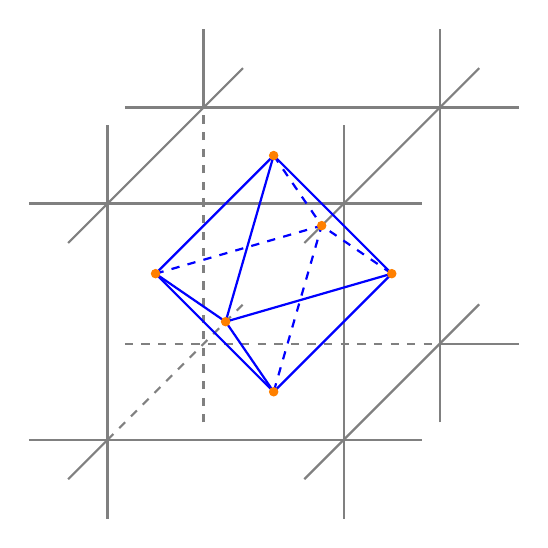
\begin{tikzpicture}
        % ---Z^3
        \draw[thick, gray] (-1, 0) -- (4, 0);
        \draw[thick, gray] (0, -1) -- (0, 4);
        \draw[thick, gray] (3, -1) -- (3, 4);
        \draw[thick, gray] (-1, 3) -- (4, 3);
        
        \draw[thick, gray, dashed] (0, 0) -- (1.72, 1.72);
        \draw[thick, gray] (-0.5, -0.5) -- (0, 0);
        \draw[thick, gray] (2.5, -0.5) -- (4.72, 1.72);
        \draw[thick, gray] (-0.5, 2.5) -- (1.72, 4.72);
        \draw[thick, gray] (2.5, 2.5) -- (4.72, 4.72);
        
        \draw[thick, gray, dashed] (1.22, 0.22) -- (1.22, 4.22);
        \draw[thick, gray] (1.22, 4.22) -- (1.22, 5.22);
        \draw[thick, gray, dashed] (0.22, 1.22) -- (4.22, 1.22);
        \draw[thick, gray] (4.22, 1.22) -- (5.22, 1.22);
        \draw[thick, gray] (4.22, 0.22) -- (4.22, 5.22);
        \draw[thick, gray] (0.22, 4.22) -- (5.22, 4.22);
        % \draw[thick] (0, 0) -- (3, 0);
        % \draw[thick] (0, 0) -- (0, 3);
        % \draw[thick] (3, 0) -- (3, 3);
        % \draw[thick] (0, 3) -- (3, 3);
        
        % \draw[thick, dashed] (0, 0) -- (1.22, 1.22);
        % \draw[thick] (3, 0) -- (4.22, 1.22);
        % \draw[thick] (0, 3) -- (1.22, 4.22);
        % \draw[thick] (3, 3) -- (4.22, 4.22);
        
        % \draw[thick, dashed] (1.22, 1.22) -- (1.22, 4.22);
        % \draw[thick, dashed] (1.22, 1.22) -- (4.22, 1.22);
        % \draw[thick] (4.22, 1.22) -- (4.22, 4.22);
        % \draw[thick] (1.22, 4.22) -- (4.22, 4.22);        
        
        % ---Z^3 dual
        
        \draw[blue, thick, dashed] (2.11, 3.61) -- (2.72, 2.72) -- (2.11, 0.61);
        \draw[blue, thick] (2.11, 3.61) -- (1.5, 1.5) -- (2.11, 0.61);
        \draw[blue, thick] (3.61, 2.11) -- (1.5, 1.5) -- (0.61, 2.11);
        \draw[blue, thick, dashed] (0.61, 2.11) -- (2.72, 2.72) -- (3.61, 2.11);
        \draw[blue, thick] (2.11, 0.61) -- (0.61, 2.11) -- (2.11, 3.61) -- (3.61, 2.11) -- (2.11, 0.61);
        
        \filldraw[orange] (1.5, 1.5) circle (1.5pt);
        \filldraw[orange] (2.72, 2.72) circle (1.5pt);
        \filldraw[orange] (2.11, 0.61) circle (1.5pt);
        \filldraw[orange] (2.11, 3.61) circle (1.5pt);
        \filldraw[orange] (0.61, 2.11) circle (1.5pt);
        \filldraw[orange] (3.61, 2.11) circle (1.5pt);
        
        % \draw[blue, thick] (1.5, 1.5) -- (2.72, 2.72);
        % \draw[blue, thick] (2.11, 0.61) -- (2.11, 3.61);
        % \draw[blue, thick] (0.61, 2.11) -- (3.61, 2.11);
        
        % \draw[cyan] (2.11, 3.61) -- (2.23, 4.03);
        % \draw[cyan] (2.11, 3.61) -- (1.81, 3.91);
        % \draw[cyan] (2.11, 3.61) -- (2.41, 3.91);
        % \draw[cyan] (2.11, 3.61) -- (1.99, 3.79);
        % \draw[cyan] (2.11, 3.61) -- (1.71, 3.61);
        % \draw[cyan] (2.11, 3.61) -- (2.51, 3.61);
        % \draw[cyan] (2.11, 3.61) -- (2.52, 4.02);
        % \draw[cyan] (2.11, 3.61) -- (1.70, 3.20);
        
    \end{tikzpicture}
    \caption{A $2 \times 2$ section of the simple cubic lattice (gray) and its dual (orange, blue)}
    \label{fig:z3_dual}
\end{figure}

We can see from \cref{fig:z3_dual} above that the dual of a cube is a regular octahedron. Moreover, consider the top vertex of the octahedron. It corresponds to the top face of the cube, whose $4$ edges each separate it from $3$ other faces. As a result, the top vertex in the dual graph is connected to $12$ other vertices, while in $\Z^3$ each vertex is connected to only $6$ neighbours. Clearly, the cubic lattice is not isomorphic to its dual. As a direct consequence, we cannot identify a one-to-one correspondence between the edges of $\Z^3$ and of $(\Z^3)^*$ to imitate how we exploited the properties of $(\Z^2)^*$ to find an upper bound on $p_c$. In fact, the self-duality of the square lattice is a very peculiar characteristic for graphs that already hints at how $p_c$ is exactly $\frac{1}{2}$ on $\Z^2$.

Nevertheless, it is enough to make the simple remark that any percolation on $\Z^3$ contains a copy of percolation on $\Z^2$, since each ``layer'' of the cubic lattice is a copy of the square lattice. Consequently, when $p > \frac{1}{2}$ --- the critical probability on $\Z^2$ as stated in \cref{thm:pc_eq_one_half_kesten}, there exists an infinite cluster on $\Z^2$  and therefore also on $\Z^3$. We conclude that $p_c \leq \frac{1}{2}$ on the cubic lattice.
\end{proof}

\begin{rem*}
It has been numerically determined that $p_c \simeq 0.24881182$ for percolation on $\Z^3$ \autocite[1]{zhou_2014}. This value is consistent with what we have established in \cref{thm:pc_on_Z3}.
\end{rem*}

\section{Conclusion}
In this investigation, we have studied the critical probability for percolation on $\Z^2$ and $\Z^3$.

One possible way to further the investigation is to consider the values of $p_c$ on other kinds of graphs. These include trees of a fixed number of branches and triangular lattices. The former is linked to genealogical trees, and it has been mathematically shown that the probability of extinction of family names is $93\%$ \autocite[]{gennes_2000} for instance. In addition, for large values of $d$, the lattice $\Z^d$ often behaves in a similar manner to trees concerning infinite clusters \autocite[]{gennes_2000}. Studies of the latter has taken this idea of similarity between different graphs even further to suggest that some properties of percolation are conserved under certain transformations. Smirnov's proof of Cardy's formula \autocite*[1]{smirnov_2001} has sparked a recent interest in this area. At the same time, many questions and a few answers have been conceived in considering more complex systems of percolation, such as directed edges.

Another direction to pursue is a closer study of how the percolation model behaves. At the same time as the notion of the critical probability allows us to understand the macroscopic behaviour concerning the existence of infinite clusters, more questions arise: when $p > p_c$, is the infinite cluster unique? (\textit{Spoiler alert:} it is.) When $p = p_c$, does an infinite cluster exist? Kesten \autocite*[1]{kesten_1980} has shown that for bond percolation on $\Z^2$, it is true that $\theta(p) = 0$. It remains an open question whether such is the case for lattices in higher dimensions, as when $p$ approaches $p_c$, the percolation system becomes fractal.

At last, we shall return to the the mathematical model itself, whose intricacy is concealed behind its simplistic formulation. Moreover, it is often difficult, if not impossible, to turn our intuition into logic. These ideas are perhaps best summed up in Kesten's words:

\begin{quotation}
``Quite apart from the fact that percolation theory had its origin in an honest applied problem, it is a source of fascinating problems of the best kind a mathematician can wish for: problems which are easy to state with a minimum of preparation, but whose solutions are (apparently) difficult and require new methods.''
\end{quotation}

\printbibliography

\end{document}
